% !Mode:: "TeX:UTF-8"

\chapter{Accelerating FDTD by Using princess VP}

In this chapter, we use the simulation of 2D TM mode as an instance to explain the scheme of accelerating FDTD by using vector processor.

\section{Data Parallelism and VP}

The vector operations, which means processing several data with one operation simultaneously, like inner production, are always used by people. Note that A one-dimensional array of numbers that packed in vector processor is called as a vector, against the scalar which includes only one number, not what is fully described by both a magnitude and a direction in physics. The terms vector and scalar address only the number of data. There are scalar processor and vector processor in CPU, which illustrated in Fig. \ref{ch3 fig:vectorprocessor}. Through the Fig. \ref{ch3 fig:vectorprocessor}, we can see that 4 numbers can be operated at the same time in a vector processor while just one number can be processed in scalar processor. 

\begin{figure}[hbtp]
\centering
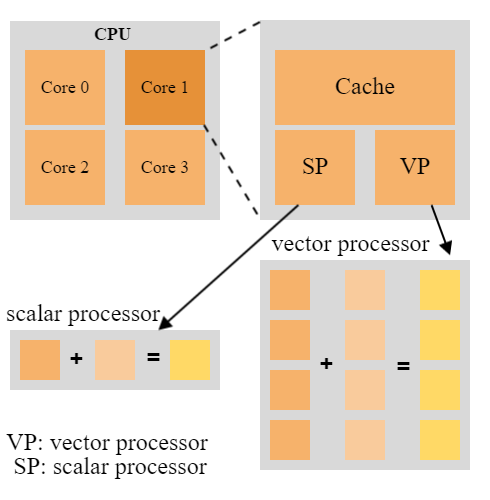
\includegraphics[width=0.7\linewidth]{pics/vectorprocessor}
\caption{Vector processor and scalar processor}
\label{ch3 fig:vectorprocessor}
\end{figure}

VP is a central processor unit that can operate vectors by a set of specific instructions. Several data are packed in some vectors by using instructions, and sent to VP. After being processed with desired operations, those vectors are sent to memory.

However, there is one important point we need to address that data object in memory should be aligned by 16 bytes when we creating them to increase the efficiency of data loads and stores to from the processor. So, we need to allocate memory suitably aligned in 16 bytes other other number of bytes designed by CPU manufacturer at the beginning of a program. If 4 contiguous float data without the first one aligned by 16 bytes, they could also be loaded into the processor, but they still should continuous in memory, and it will be slower by 4.5 times than aligned situation.

\section{The Scheme of Accelerating FDTD by Using VP}

Taking TM mode as example, the discrete form of updating formulations of the field vector components $H_x$, $H_y$, and $E_z$ are as following:
\begin{equation}\label{ch3: hx}
H^{n+\frac{1}{2}}_{x}\left(i,j+\frac{1}{2}\right)=H^{n-\frac{1}{2}}_{x}\left(i,j+\frac{1}{2}\right)+
\frac{\Delta t}{\mu}\left(
\frac{E^n_z(i,j)-E^n_z(i,j+1)}{\Delta y}
\right)
\end{equation}
\begin{equation}
H^{n+\frac{1}{2}}_{y}\left(i+\frac{1}{2},j\right)=H^{n-\frac{1}{2}}_{y}\left(i+\frac{1}{2},j\right)+
\frac{\Delta t}{\mu}\left(
\frac{E^n_z(i+1,j)-E^n_z(i,j)}{\Delta x}
\right)
\end{equation}
\begin{equation}\label{ch3: ez}
\begin{split}
E^{n+1}_z(i,j)=&E_z^n(i,j)\\
&+\frac{\Delta t}{\epsilon}\left(
\frac{H_y^{n+1/2}(i+\frac{1}{2},j)-H_y^{n+1/2}(i-\frac{1}{2},j)}{\kappa_x \Delta x}\right.\\
&\left.-\frac{H_x^{n+1/2}(i,j+\frac{1}{2})-H_x^{n+1/2}(i,j-\frac{1}{2})}{\kappa_y \Delta y}
\right)
\end{split}
\end{equation}

The next, we take a 3$\times$3 size grids as an instance to explain the traditional data parallelism scheme intuitively. According to the way of Fig. \ref{ch2 fig: yee cell}, we position all field vector components as what shown in the Fig. \ref{ch3 fig:2d yee} in the $3\times3$ size Yee cells. The serial numbers in grids represent the position of the corresponding discrete field point, which the position in $y$ direction, ie the row it is on, is represented by the first number of a serial number, and correspondingly, the position in $x$ deirection, ie the column it is on, is represented by the second number of a serial number.

\begin{figure}[hp]
	\centering
	\def \xcells {7}
	\def \ycells {7}
	\def \cell {1.2}
	\begin{tikzpicture}
	%\draw (0,0) grid (\xcells,\ycells);
	%Ez
	\foreach \x in {0,1,2,3}{
		\foreach \y in {0,1,2,3}{
			\filldraw[yellow] (2*\y,2*\x) rectangle (2*\y+1,2*\x+1);
			\node at (2*\y+0.5,2*\x+0.5) {\x,\y};
		}	
	}
	%grid
	\foreach \x in {1,3,5}{
		\foreach \y in {1,3,5}{
			\filldraw[lightgray] (\x,\y) rectangle (\x+1,\y+1);
		}	
	}
	%Hy
	\foreach \x in {0,1,2,3}{
		\foreach \y in {0,1,2}{
			\filldraw[pink] (2*\x,2*\y+1) rectangle (2*\x+1,2*\y+2);
			\node at (2*\x+0.5,2*\y+1.5) {\y,\x};
		}	
	}
	%Hx
	\foreach \x in {0,1,2}{
		\foreach \y in {0,1,2,3}{
			\filldraw[cyan] (2*\x+1,2*\y) rectangle (2*\x+2,2*\y+1);
			\node at (2*\x+1.5,2*\y+0.5) {\y,\x};
		}	
	}
	\draw [-stealth] (0,0) -- (\xcells+1,0) node[right] {$x$};
	\draw [-stealth] (0,0) -- (0,\ycells+1) node[right] {$y$};
	
	\filldraw[cyan] ($(0,-2)$) rectangle ($(0,-2)+(\cell,\cell)$);
	\node at ($(0,-2)+0.5*(\cell,\cell)$) {$H_x$};
	
	\filldraw[pink] ($(\cell,-2)$) rectangle ($(\cell,-2)+(\cell,\cell)$);
	\node at ($(\cell,-2)+0.5*(\cell,\cell)$) {$H_y$};
	
	\filldraw[yellow] ($(2*\cell,-2)$) rectangle ($(2*\cell,-2)+(\cell,\cell)$);
	\node at ($(2*\cell,-2)+0.5*(\cell,\cell)$) {$E_z$};
	
	\filldraw[lightgray] ($(3*\cell,-2)$) rectangle ($(3*\cell,-2)+(\cell,\cell)$);
	\node [align=center] at ($(3*\cell,-2)+0.5*(\cell,\cell)$) {Yee\\网格};
	\end{tikzpicture}
	\caption{The position of discrete field points in Yee cells of TM mode wave}
	\label{ch3 fig:2d yee}
\end{figure}

The traditional data parallelism method of FDTD, did some modifications, which is adding some auxiliary $H_x$ field points at the boundary of $x$ direction, to the spatial organization shown in Fig. \ref{ch3 fig:2d old}. Now, let $N_x$ and $N_y$ are the number of Yee cell of $x$, $y$ direction respectively. Therefore, the number of discrete field points of each field vector component are shown as Table \ref{ch3 table: old number}.

\begin{figure}
	\centering
	\def \xcells {7}
	\def \ycells {7}
	\def \cell {1.2}
	\begin{tikzpicture}
	%\draw (0,0) grid (\xcells,\ycells);
	%Ez
	\foreach \x in {0,1,2,3}{
		\foreach \y in {0,1,2,3}{
			\filldraw[yellow] (2*\y,2*\x) rectangle (2*\y+1,2*\x+1);
			\node at (2*\y+0.5,2*\x+0.5) {\x,\y};
		}	
	}
	%grid
	\foreach \x in {1,3,5}{
		\foreach \y in {1,3,5}{
			\filldraw[lightgray] (\x,\y) rectangle (\x+1,\y+1);
		}	
	}
	%Hy
	\foreach \x in {0,1,2,3}{
		\foreach \y in {0,1,2}{
			\filldraw[pink] (2*\x,2*\y+1) rectangle (2*\x+1,2*\y+2);
			\node at (2*\x+0.5,2*\y+1.5) {\y,\x};
		}	
	}
	%Hx
	\foreach \x in {0,1,2,3}{
		\foreach \y in {0,1,2}{
			\filldraw[cyan] (2*\x+1,2*\y) rectangle (2*\x+2,2*\y+1);
			\node at (2*\x+1.5,2*\y+0.5) {\y,\x};
		}	
	}
	\draw [-stealth] (0,0) -- (\xcells+2,0) node[right] {$x$};
	\draw [-stealth] (0,0) -- (0,\ycells+1) node[right] {$y$};
	
	\filldraw[cyan] ($(0,-2)$) rectangle ($(0,-2)+(\cell,\cell)$);
	\node at ($(0,-2)+0.5*(\cell,\cell)$) {$H_x$};
	
	\filldraw[pink] ($(\cell,-2)$) rectangle ($(\cell,-2)+(\cell,\cell)$);
	\node at ($(\cell,-2)+0.5*(\cell,\cell)$) {$H_y$};
	
	\filldraw[yellow] ($(2*\cell,-2)$) rectangle ($(2*\cell,-2)+(\cell,\cell)$);
	\node at ($(2*\cell,-2)+0.5*(\cell,\cell)$) {$E_z$};
	
	\filldraw[lightgray] ($(3*\cell,-2)$) rectangle ($(3*\cell,-2)+(\cell,\cell)$);
	\node [align=center] at ($(3*\cell,-2)+0.5*(\cell,\cell)$) {Yee cell};
	\end{tikzpicture}
	\caption{The computational model of traditional data parallelism method}
	\label{ch3 fig:2d old}
\end{figure}


\begin{table}[hp]
\centering
\caption{The number of discrete points of each field component in each direction}
\label{ch3 table: old number}
\begin{tabular}{ccc}
	\toprule
	Field component & The number in $x$ direction & The number in $y$ direction\\
	
	\midrule
	$E_z$ & $N_x+1$ & $N_y+1$\\
	$H_x$ & $N_x+1$ & $N_y$\\
	$H_y$ & $N_x+1$ & $N_y$\\
	\bottomrule
\end{tabular}
\end{table}

In the program, we allocate a block of memory whose addresses are continuous and size is corresponding the number of the field component whose data is stored in it. For example, in the 3$\times$3 Yee cell, we allocate three blocks of memory which can store 16 floats, 12 floats, 12floats, to store the data of $E_z$, $H_x$, and $H_y$ respectively. Besides, we follow the rule that all field vector components are growing in the $x$ direction first, ie the second number of the serial number growing first. So, take discrete field points of $E_z$ as an example, they are stored in the memory in a one-dimension way, and their serial numbers are $(0,0)\cdots(0,3),(1,0)\cdots$.

The process of computing field vector components, here, we explicate it by taking computing $H_x$ as an example, without specify the instruction set used. The first step, load three vectors according to the equation \eqref{ch3: hx}. The first vector, including the first five discrete points of $H_x$, ie $H_x(0,0)$ to $H_x(1,0)$, is noted as $V_{H_x}$. The second vector, including the first five discrete points of $E_z$, ie $E_z(0,0)$ to $E_z(1,0)$, is noted as $V_{E_z}^1$. The third vector, including five continuous discrete points of $E_z$ from the second points, ie $E_z(0,1)$ to $E_z(1,1)$, is noted as $V_{E_z}^2$.

The second step, we use instructions to have $V_{E_z}^1$ minus $V_{E_z}^2$, and note the result as $V_{sub}$. More specifically speaking, let the first data of the $V_{E_z}^1$, minus the first data of $V_{E_z}^2$, and so on. Then, all data of $V_{sub}$ multiply the constant, $\frac{\Delta t}{\mu\Delta x}$, and the result is noted as $V_{sub}^{'}$. At last, let $V_{sub}^{'}$ add $V_{H_x}$, to get the final consequence. So, we implement equation \eqref{ch3: hx}. Repeating this step over all discrete points of $H_x$. The process is illustrated in Fig. \ref{ch3 fig:cmp}.

The last step, is to store those elements of vectors back to memory, a reverse to the first step.

\begin{figure}[hbtp]
\centering
\def \yshift {-1}
\def \xshift {1}
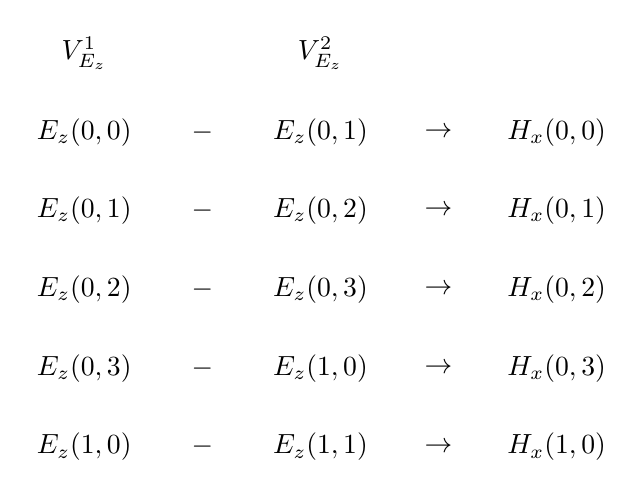
\begin{tikzpicture}

\node at (0,0) {$E_z(0,0)$};
\node at (0,\yshift) {$E_z(0,1)$};
\node at (0,2*\yshift) {$E_z(0,2)$};
\node at (0,3*\yshift) {$E_z(0,3)$};
\node at (0,4*\yshift) {$E_z(1,0)$};

\foreach \y in {0,1,2,3,4}{
	\node at (\xshift,\y*\yshift) {$-$};	
}

\node at (2*\xshift,0) {$E_z(0,1)$};
\node at (2*\xshift,\yshift) {$E_z(0,2)$};
\node at (2*\xshift,2*\yshift) {$E_z(0,3)$};
\node at (2*\xshift,3*\yshift) {$E_z(1,0)$};
\node at (2*\xshift,4*\yshift) {$E_z(1,1)$};

\foreach \y in {0,1,2,3,4}{
	\node at (3*\xshift,\y*\yshift) {$\rightarrow$};	
}

\node at (4*\xshift,0) {$H_x(0,0)$};
\node at (4*\xshift,\yshift) {$H_x(0,1)$};
\node at (4*\xshift,2*\yshift) {$H_x(0,2)$};
\node at (4*\xshift,3*\yshift) {$H_x(0,3)$};
\node at (4*\xshift,4*\yshift) {$H_x(1,0)$};

\node at (0,-\yshift) {$V_{E_z}^1$};
\node at (2*\xshift,-\yshift) {$V_{E_z}^2$};
\end{tikzpicture}
\caption{The process of computing $H_x$ in traditional scheme}
\label{ch3 fig:cmp}
\end{figure}

From the Fig. \ref{ch3 fig:cmp}, we can see that one of those auxiliary points, ie $H_x(0,3)$, keep all elements in those three vector having a constant relationship, which allows us process those elements by one instruction at one time. In Fig. \ref{ch3 fig:cmp}, the constant relationship is the serial numbers of one set of points of $E_z$ are the same as the serial number of the set of points $H_x$, while the serial numbers of another set of points of $E_z$, are bigger by 1 on two parts of serial numbers. If we remove those auxiliary points, we need to add some code to find out which field points we should load in VP, and compute less than 4 points by using scalar processor in each row. Those extra process will make program more complex and fewer efficient.

\section{A New Computational Model for Data Parallelism}

In the traditional parallel FDTD method, the computational model derived directly from Yee cell showed in Fig. 3 is adaptable to almost all boundary conditions. Nevertheless, for some specific boundary conditions, like PEC and MUR, we can modify the model of the traditional data parallel method. 

Let us take a look on PEC boundary condition first. PEC boundary condition is a TBC. In PEC, we set all electric field points are 0. ie
\begin{equation}\label{ch3: pec}
E(k)=0,
\end{equation}
in which $E(k)$ represent the discrete electric field points on boundaries.

The Mur ABC, "absorbing" waves without any reflection when they arrive at the boundary of simulation area's boundaries. Consider the homogeneous equation in one-dimension form:
\begin{equation}
\frac{\partial^2 u}{\partial x^2}-\frac{1}{c^2}\frac{\partial^2 u}{\partial t^2}=0.
\end{equation}\label{ch3 eq:homogeneous 1D}
The solution to equation \eqref{ch3 eq:homogeneous 1D} is
\begin{equation}
u(x,t)=A\exp[j(\omega t-k_x x)].
\end{equation}

Set $x=0$ is the left boundary. For there are incident wave and reflected wave, so we have
\begin{equation}
u(x,t)=A_{-}\exp[j(\omega t+k_x x)]+A_{+}\exp[j(\omega t-k_x x)].
\end{equation}
Note the first and second term of the right side is $u_{-}$ and $u_{+}$ respectively. If we want to remove the reflected wave, we should set $u_{+}$  to be 0. Hence, there has
\begin{equation}
\frac{\partial u}{\partial x}-\frac{1}{c}\frac{\partial u}{\partial t}=0.
\end{equation}\label{ch3 eq:reflected wave be 0}

By discretizing equation \eqref{ch3 eq:reflected wave be 0}, we have
\begin{equation}\label{ch3: mur}
u^{n+1}(k)=u^n(k-1)+\frac{c\Delta t-\Delta z}{c\Delta t+\Delta z}[u^{n+1}(k-1)-u^n(k)],
\end{equation}
In which $u(k)$ represent boundary points, $u(k-1)$ represent the points close to the $u(k)$.

According to equation \eqref{ch3: pec} and \eqref{ch3: mur}, discrete points of other field vector component are not need to compute those points of electric field and on boundaries. Therefore we can simplify the computational model, it the spatial organization shown in Fig. \ref{ch2 fig: yee cell} by remove some magnetic field points between those electric field points which on boundary. By doing this, the number of discrete points need to be computed is reduced. Here, we still use the 3$\times$3 Yee cell grid to explain our modified computational model, which shown in Fig. \ref{ch3 fig:2d new}.

\begin{figure}[hp]
	\centering
		\def \xcells {7}
		\def \ycells {7}
		\def \cell {1.2}
	\begin{tikzpicture}
	%\draw (0,0) grid (\xcells,\ycells);
	%Ez
	\foreach \x in {0,1,2,3}{
		\foreach \y in {0,1,2,3}{
			\filldraw[yellow] (2*\y,2*\x) rectangle (2*\y+1,2*\x+1);
			\node at (2*\y+0.5,2*\x+0.5) {\x,\y};
		}	
	}
	%grid
	\foreach \x in {1,3,5}{
		\foreach \y in {1,3,5}{
			\filldraw[lightgray] (\x,\y) rectangle (\x+1,\y+1);
		}	
	}
	%Hy
	\foreach \x in {0,1}{
		\foreach \y in {0,1,2}{
			\filldraw[pink] (2*\x+2,2*\y+1) rectangle (2*\x+3,2*\y+2);
			\node at (2*\x+2.5,2*\y+1.5) {\y,\x};
		}	
	}
	%Hx
	\foreach \x in {0,1,2}{
		\foreach \y in {0,1}{
			\filldraw[cyan] (2*\x+1,2*\y+2) rectangle (2*\x+2,2*\y+3);
			\node at (2*\x+1.5,2*\y+2.5) {\y,\x};
		}	
	}
	\draw [-stealth] (0,0) -- (\xcells+1,0) node[right] {$x$};
	\draw [-stealth] (0,0) -- (0,\ycells+1) node[right] {$y$};
	
	\filldraw[cyan] ($(0,-2)$) rectangle ($(0,-2)+(\cell,\cell)$);
	\node at ($(0,-2)+0.5*(\cell,\cell)$) {$H_x$};
	
	\filldraw[pink] ($(\cell,-2)$) rectangle ($(\cell,-2)+(\cell,\cell)$);
	\node at ($(\cell,-2)+0.5*(\cell,\cell)$) {$H_y$};
	
	\filldraw[yellow] ($(2*\cell,-2)$) rectangle ($(2*\cell,-2)+(\cell,\cell)$);
	\node at ($(2*\cell,-2)+0.5*(\cell,\cell)$) {$E_z$};
	
	\filldraw[lightgray] ($(3*\cell,-2)$) rectangle ($(3*\cell,-2)+(\cell,\cell)$);
	\node [align=center] at ($(3*\cell,-2)+0.5*(\cell,\cell)$) {Yee\\cell};
	\end{tikzpicture}
	\caption{The modified computational model of data parallelism}
	\label{ch3 fig:2d new}
\end{figure}

From the Fig. \ref{ch3 fig:2d new} we can see that all magnetic field points outside the Yee cell grids area are removed. Now,  the number of discrete field points of each field vector component are shown as Table \ref{ch3 table:new number}. Also let $N_x$ and $N_y$ are the number of Yee cell of $x$, $y$ direction respectively.

\begin{table}[hp]
	\centering
	\caption{The number of discrete points of each field component in each direction in new computational model}
	\label{ch3 table:new number}
	\begin{tabular}{ccc}
		\toprule
		Field component & The number in $x$ direction & The number in $y$ direction\\
		
		\midrule
		$E_z$ & $N_x+1$ & $N_y+1$\\
		$H_x$ & $N_x$ & $N_y-1$\\
		$H_y$ & $N_x-1$ & $N_y$\\
		\bottomrule
	\end{tabular}
\end{table}

In the program, the same with what we doing in traditional scheme, we allocate a block of memory whose addresses are continuous and size is corresponding the number of the field component whose data is stored in it. For example, in the 3$\times$3 Yee cell, we allocate three blocks of memory which can store 16 floats, 6 floats, 6 floats, to store the data of $E_z$, $H_x$, and $H_y$ respectively. Besides, we also follow the rule that all field vector components are growing in the $x$ direction first, ie the second number of the serial number growing first.

In the traditional computational model, with those auxiliary $H_x$ points, the physical position of a data in memory is uniform to its logical position, ie the m-th float stored in three blocks memory are $E_z(y_m,x_m)$, $H_x(y_m,x_m)$, and $H_y(y_m,x_m)$. However, in the modified new computational model things get changed. So, taking the computation of $H_x$ as example again. According the steps stated in the last section, when we want to compute the first four points of $H_x$, we need to load three vectors in VP. They are $V_{H_x}$, including $H_x(0,0)$ to $H_x(1,0)$; $V_{E_z}^1$, including $E_z(1,0)$ to $E_z(1,3)$; and $V_{E_z}^2$, including $E_z(1,1)$ to $E_z(2,0)$. Following the process mentioned in the last section, let the $V_{E_z}^1$ minus $V_{E_z}^2$. You will find there are something wrong here: The $E_z(2,0)$ will minus $E_z(1,3)$. However, according to the equation \eqref{ch3: hx}, we need $E_z(2,1)$ to minus $E_z(2,0)$ if we want to update the value of $H_x(1,0)$.

As things are becoming different now, we have to do two modifications. The first, we can no more apply one process over all points of a field vector component. We should divide a rwo into several separate sections and do different processes on them separately, too. The second, we should understand that not all points can be computed by VP, now. We should note that some special points, like some point on head or tail of a row.

\section{The Comparison between Traditional and Modified Computational Model}

In this paper, we take the computation of 2D FDTD TM wave using Mur ABC as an example to analyze the difference between using data parallelism or not, the traditional and our modified method, and the performance of the modified method in different space and time sizes. Furthermore, we analyze the efficiency of those two methods based on those results.

The framework of the program is presented in the function’s call tree form, which is illustrated in Fig. \ref{ch3 workflow:calltree}. From it, we can see that the program consists of 3 parts which are input, response to initialize data; \lstinline|H\_cmp| and \lstinline|E\_cmp|, two functions that compute electromagnetic field; and other functions that dealing with other things. Once we run the code, the Input works first and then are \lstinline|H\_cmp| and \lstinline|E\_cmp| which are called iterating, the last,other functions do some auxiliary works like saving the result of the computation to files.

\begin{figure}
	\centering
	\tikzstyle{box} = [rectangle, rounded corners, minimum width = 1cm,text centered, draw=black,align=center]
	\tikzstyle{arrow} = [thick,->,>=stealth]
	\begin{tikzpicture}
	\def \yshift {-1cm}
	\def \xshift {1.5cm}
	\node (main) [box] {\lstinline|main|};
	\node (input) [box,right of= main,yshift=-\yshift,xshift=\xshift] {\lstinline|input|};
	\node (compute) [box,right of=main,yshift=\yshift,xshift=\xshift] {\lstinline|compute|};
	\node (hcmp) [box,right of = compute,yshift=-\yshift,xshift=\xshift] {\lstinline|H_cmp|};
	\node (ecmp) [box,right of = compute,xshift=\xshift] {\lstinline|E_cmp|};
	\node (other) [box,right of = compute,yshift=\yshift,xshift=\xshift] {其它};
	
	\draw (main) --++(0.5*\xshift,0)--+(0,-\yshift)-- (input);
	\draw (main) --++(0.5*\xshift,0)--+(0,\yshift)-- (compute);
	\draw (compute) --++(\xshift,0)--+(0,-\yshift)-- (hcmp);
	\draw (compute) --++(\xshift,0)--+(0,\yshift)-- (other);
	\draw (compute) -- (ecmp);
	\draw [arrow] (input) -- (compute);
	\draw [arrow] (hcmp) -- (ecmp);
	\draw [arrow] (ecmp) -- (other);
	\end{tikzpicture}
	\caption{The framework of the program}
	\label{ch3 workflow:calltree}
\end{figure}

We adopted the methods provided by Visual Studio Profiling Tools to collect the performance data of sample project and analyze them. There are two kinds of profiling methods we were using. The first is sampling
profiling method, and another is instrumentation profiling method. The sampling profiling method collects statistical data about an application, including the function call stack. The instrumentation profiling method collects detailed timing for the function calls in a profiled application. 


Instrumentation use four types of values to represent the time spent in a function or source code line and here we use two of them, which are:
\begin{description}
	\item[Elapsed Inclusive]\quad The total time that is spent to execute the function or source line.
	\item[Elapsed Exclusive]\quad The time that is spent executing code in the body of the function or source code line. Time that is spent executing functions that are called by the function or source line is excluded.%reference
\end{description}

So, in our program, the elapsed inclusive time of function \lstinline|main| represent the time elapsed by the whole program; the elapsed inclusive time of function \lstdefinestyle{compute} represent the time elapsed to compute all discrete field points; as \lstinline|H_cmp| and \lstinline|E_cmp| do not call other functions, so the elapsed inclusive and exclusive time are equal and all represent the average time spent on those two functions. In fact, for function \lstinline|H_cmp| and \lstinline|E_cmp|, we concern exactly the time spent in one time.

We also use Release option to see the differences more clearly, as by doing this we can ignore some minor problems caused by accident or bad programming habit. Besides, to guarantee the accuracy of the analysis, for every condition we ran the program for five times and obtain the average value of those profiling results. The configuration is Intel Core i5-3210M 2.3GHz, 4.00GB memory, Windows 10 64-bits and Visual Studio 2015.

The following tables give out the performances of traditional scheme and our modified scheme which using new computational model under different condition.

\begin{table}[hp]
\centering
\begin{threeparttable}
	\caption{The comparison between using data parallelism or not}\label{ch3: data parallel or not}
	\begin{tabular}{cccc}
		\toprule
		\multirow{2}{3em}{Function}&\multicolumn{2}{c}{Elapsed Exclusive (ms)} & \multirow{2}{11em}{Time saved by using data parallelism}\\
		\cline{2-3}
		& No parallelism & New model & \\ 
		
		\midrule
		\lstinline|main| & 10330.43 & 7835.78 & 24.15\% \\ 
		\lstinline|compute| & 10313.62 & 7819.76 & 24.18\%\\ 
		\lstinline|H_cmp|& 6.16 & 4.64 & 24.62\%\\ 
		\lstinline|E_cmp|& 4.10 & 3.13 &23.78\% \\
		\bottomrule
	\end{tabular} 
	\begin{tablenotes}
		\item[1] The size of simulation area is 2000$\times$1000 Yee cells.
		\item[2] The number of time step is 1000.
	\end{tablenotes}
\end{threeparttable}
\end{table}

According to Table \ref{ch3: data parallel or not}. The whole running time of \lstinline|H_cmp| and \lstinline|E_cmp| are obtained by multiplying the time steps with the Average Elapsed Exclusive Time. We can see easily after some simple calculations that the time
spent by those two functions are 6160ms and 4100ms, over 99.3\% and 99.2\% of the time spent by the whole program respectively. Hence, we can say safely that the differences between two methods are mainly caused by the \lstinline|H_cmp| and \lstinline|E_cmp|. According to the Table 2, the time-consuming of FDTD method had been reduced about by 24\%. It shows us that data parallelism can enhance the efficiency of FDTD largely.

\begin{table}[hp]
\centering
\caption{The comparison between traditional and new computational model}\label{ch3: tradition or new}
\begin{threeparttable}
	\begin{tabular}{cccc}
		\toprule
		\multirow{2}{3em}{Function}&\multicolumn{2}{c}{Elapsed Inclusive (ms)} & \multirow{2}{11em}{Time saved by using new model}\\ 
		\cline{2-3}
		& Traditional model & New model & \\ 
		
		\midrule
		\lstinline|main| & 4229.46 & 4082.64 & 3.47\% \\ 
		\lstinline|compute| & 4216.81 & 4070.73 & 3.46\%\\ 
		\lstinline|H_cmp|& 2.50 & 2.41 & 3.37\%\\ 
		\lstinline|E_cmp|& 1.68 & 1.62 & 3.57\% \\
		\bottomrule
	\end{tabular}
	\begin{tablenotes}
		\item[1] The size of simulation area is 1000$\times$1000 Yee cells.
		\item[2] The number of time step is 1000.
	\end{tablenotes}
\end{threeparttable}
\end{table}

What we can see from the Table \ref{ch3: tradition or new} is that the elapsed time of the whole program by using new computational had been saved about by 3.45\% compared to the traditional model. With the analysis we did above, the conclusion can be concluded that the computational model of the new methods is better than that of the traditional method. Though some discrete field points are computed by scalar processor, which is a drawback, but the reduction of the number of whole discrete points which means less points the processor need to compute, not only compensate the waste caused by that drawback, but also make the elapsed time shorter.

\begin{table}[hp]
	\centering
	\begin{threeparttable}
	\caption{The performance of new model under different space size}\label{ch3: new, size}
		\begin{tabular}{cccc}
			\toprule
			\multirow{2}{3em}{Function}&\multicolumn{3}{c}{Elapsed Inclusive (ms)}\\ 
			\cline{2-4}
			& $1000\times1000$ & $2000\times1000$ & $3000\times1000$\\ 
			
			\midrule
			\lstinline|main| & 4082.64 & 7835.78 & 11597.80 \\ 
			\lstinline|compute| & 4072.73 & 7819.76 & 11577.88\\ 
			\lstinline|H_cmp|& 2.412 & 4.64 & 6.87\\ 
			\lstinline|E_cmp|& 1.62 & 3.13 & 4.65 \\
			\bottomrule
		\end{tabular}
		\begin{tablenotes}
			\item[1] The number of time step is 1000.
		\end{tablenotes}
	\end{threeparttable}
\end{table}

Based on Table \ref{ch3: new, size}, we can see the time-consuming of the whole program is linear to the size of space scale. From the data we collected, when the size of space scale is as n times as before, the time-consuming will be about $0.92n+0.08$ times than before.

\begin{table}[hp]
	\centering
	\begin{threeparttable}
		\caption{The performance of new model under different time size}\label{ch3: new, time}
		\begin{tabular}{ccc}
			\toprule
			\multirow{2}{3em}{Function}&\multicolumn{2}{c}{Elapsed Inclusive (ms)}\\ 
			\cline{2-3}
			& 1000 time steps & 3000 time steps\\ 
			
			\midrule
			\lstinline|main| & 7835.78 & 23247.73 \\ 
			\lstinline|compute| & 7819.76 & 23230.83\\ 
			\lstinline|H_cmp|& 4.64 & 4.59\\ 
			\lstinline|E_cmp|& 3.13 & 3.10\\
			\bottomrule
		\end{tabular}
		\begin{tablenotes}
			\item[1] The simulation area had 2000$\times$1000 Yee cells.
		\end{tablenotes}
	\end{threeparttable}
\end{table}

From the Table \ref{ch3: new, time}, we can see that with time step increases, the average time-consuming of every time step is decreased.
The time-consuming of each time step in the 3000 steps condition is 0.99 times to that of 1000 time steps condition. We believe that this is because with the number of iteration increase, the computer can hit the memory more accurately.

\section{Conclusion}

In this chapter, the 2D TM model is taken as an instance to explain a new data parallel FDTD method which is a modification of the traditional methods and how it is advanced under MUR boundary condition with fewer boundary points that need to be compute. The new method was programmed by using C and SSE. Besides, based on the profiling results by running the program for different conditions like the different sizes of simulation space and time, the performance data of the new method and the traditional method were obtained. At last, by
analyzing the performance data, the conclusion was derived that our new method saves about 3.45\% time which mean that it is better than the traditional data parallel FDTD method.